\chapter{Aktuelle Engineentwicklung}
\label{chap:engine-uebersicht}

%% Zitat:
% https://twitter.com/CompSciFact/status/527816734863265792
\epigraph{Even if your code was perfect when you released it, it still needs to be maintained because the world around it is changing.}{Unbekannt}

Spiele- und Grafikengines sind inzwischen äußerst komplexe Softwareprojekte. Früher wurden Spiele von Einzelpersonen oder kleinen Teams entwickelt, heute sind Teamstärken von über 100 Entwicklern keine Seltenheit. Komplexe Softwareprojekte erfordern neue Projektstrukturen, und dem entsprechend haben sich die Projektstrukturen im Laufe der Zeit gewandelt. Mit der Professionalisierung der Branche sind auch die Anforderungen an die Software zumindest klar definiert: Das Softwareprojekt ist langfristing angelegt, soll dem entsprechend robust und flexibel, wartbar, zugänglich und verständlich sein. Projektstrukturen sind inzwischen häufig auf kurze Iterationszyklen ausgelegt, Die dem Entwicklerteam ermöglichen sollen, auf die sich verändernde Umwelt und den neuen Anforderungen und Gegebenheiten flexibel zu reagieren.

Gerade im letzten Jahr hat sich auf dem Markt der kommerziellen Spiele- und Grafikengines einiges verändert. Die wichtigsten Entwickler von kommerziellen Engines, wie \textit{Epic Games}, \textit{Unity} oder \textit{Crytek}, haben ihre Projekte der Allgemeinheit geöffnet, während früher noch sechsstellige Beträge für den Einblick in den Quelltext zu zahlen waren. Inzwischen rufen die Entwickler direkt zur Mitarbeit an ihrer Engine auf. Das bringt für beide Seiten Vorteile. Zwar muss der beitragende Entwickler auf seine Rechte am Code verzichten\footnote{https://www.unrealengine.com/eula}, doch kann er direkten Einfluss auf Entwicklung nehmen. Und auf der anderen Seite kann das Unternehmen den Eifer der Entwickler kommerziell verwerten aber auch neue fähige Mitarbeiter rekrutieren.

Zusätzlich hat sich der Fokus der aktuellen Engines deutlich verschoben. Während noch vor ein paar Jahren die Editoren noch recht komplex zu bedienen waren und meist immer noch tiefergehende Programmierkenntnisse erforderlich waren, sind die aktuellen Editoren deutlich einsteigerfreundlicher geworden. Erste Prototypen oder einfache Spiele sind in Editoren wie dem \textit{UnrealEd} über das Blueprint genannte System ohne eigentliche Programmierkenntnisse umsetzbar. Komplexere und spezifische Blueprints werden später wieder von den Programmierern umgesetzt, die dann von Game-Designer zur Anwendung gebracht werden können.

\begin{figure}
\centering
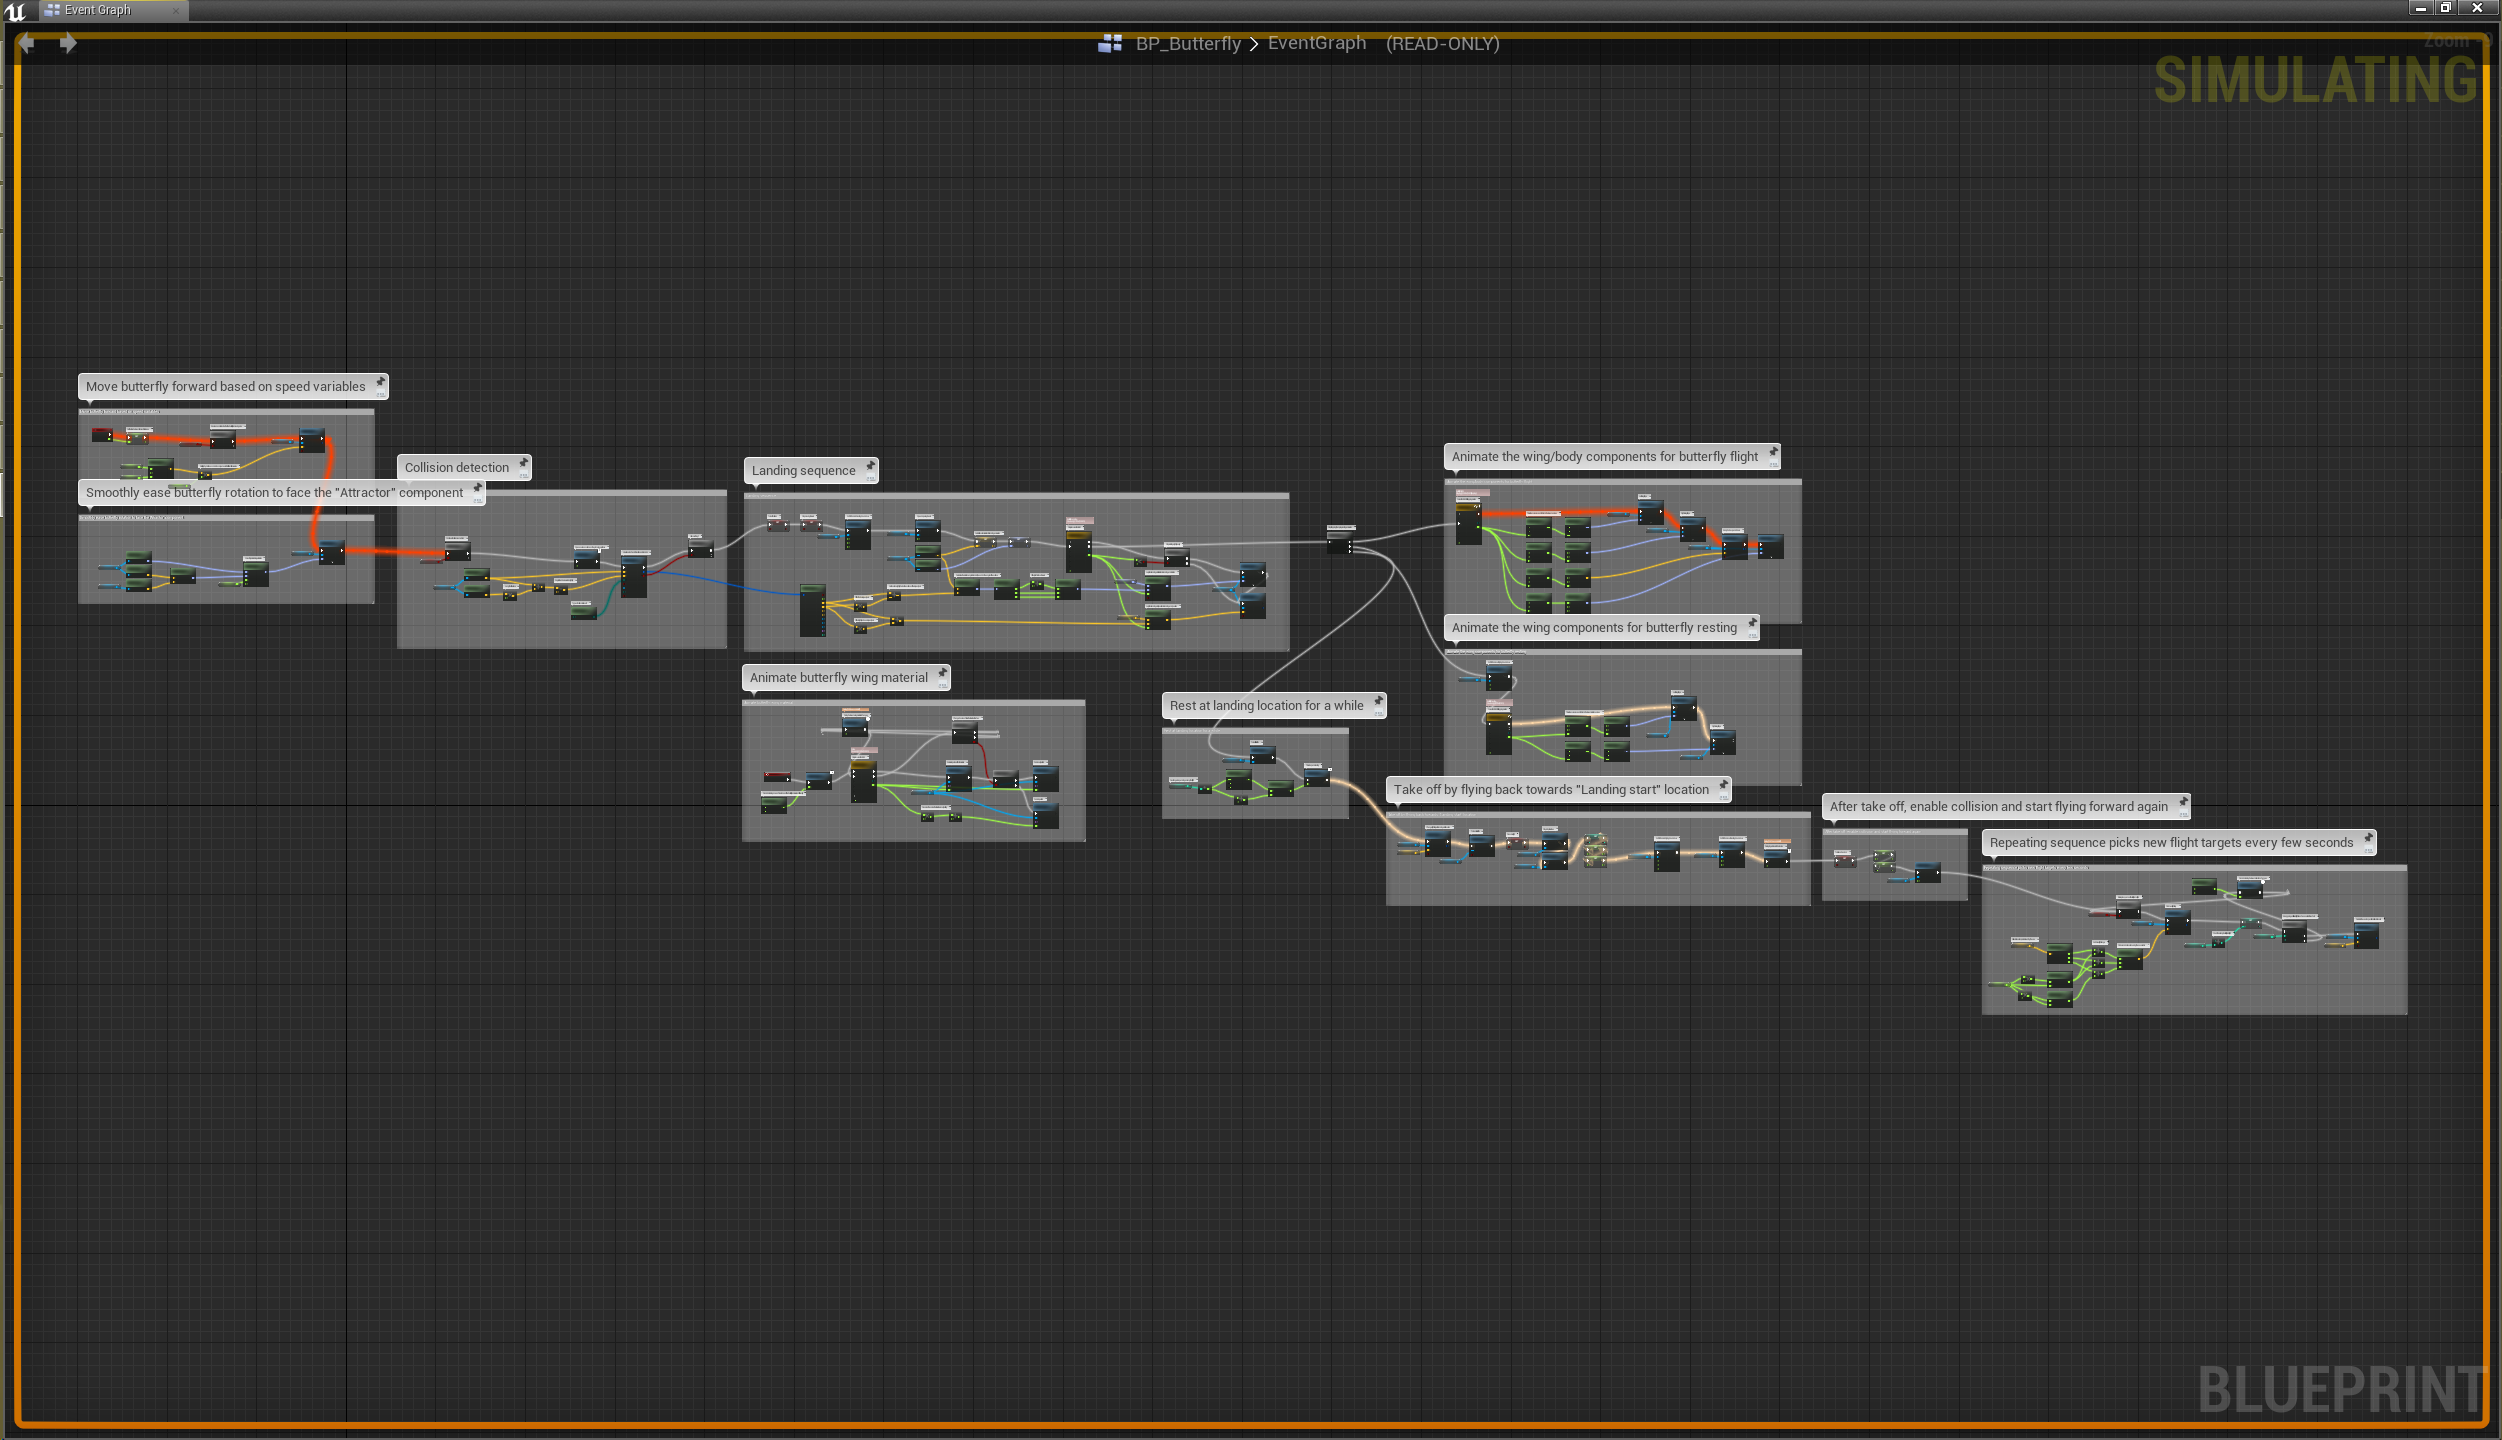
\includegraphics[width=\textwidth]{ue4-blueprint}
\caption{Unreal Engine 4 Blueprint Beispiel}
\end{figure}

\section{Grafik Engines in Haskell}
http://www.hgamer3d.org/
https://lambdacube3d.wordpress.com/
Gloss (2d)
